\capitulo{3}{Conceptos teóricos}


\section{ Importancia de la calidad del sueño}

El sueño es un proceso biológico fundamental para la regulación de múltiples funciones fisiológicas, cognitivas y metabólicas. Su importancia radica en su papel en la homeostasis del organismo, la consolidación de la memoria, la regulación del estado anímico y la prevención de enfermedades crónicas. Estudios epidemiológicos han demostrado que una deficiencia en la calidad del sueño está asociada con un mayor riesgo de enfermedades cardiovasculares, metabólicas y psiquiátricas, así como con una reducción en el rendimiento cognitivo y una mayor incidencia de accidentes laborales y de tráfico  \cite{interactions}.

Desde el punto de vista fisiológico, el sueño se estructura en ciclos de aproximadamente 90 a 120 minutos que se repiten durante la noche, alternando entre dos grandes fases: sueño NREM (no REM) y sueño REM (movimientos oculares rápidos). El \textbf{sueño NREM} comprende tres estadios (N1, N2 y N3) según la clasificación actual de la AASM\footnote{Según la Academia Estadounidense de Medicina del Sueño: \url{https://aasm.org/}.}, que van desde el sueño ligero hasta el sueño profundo, asociado a la recuperación física y a la secreción de hormonas como la del crecimiento. Por su parte, el \textbf{sueño REM} se caracteriza por una intensa actividad cerebral, sueños vívidos y consolidación de la memoria emocional. La correcta alternancia entre estas fases es clave para un descanso reparador, y su alteración se ha relacionado con diversas patologías físicas y mentales \cite{sleepfoundation2023}.


\subsection{Impacto en la Funcionalidad Cognitiva}


El sueño profundo y, especialmente, la fase REM, desempeñan un papel esencial en la consolidación de la memoria y en procesos clave de aprendizaje. Según estudios en neurociencia, la privación del sueño disminuye la plasticidad neuronal y afecta negativamente a la consolidación de la memoria declarativa y procedimental \cite{funcionCognitiva}. Stickgold y Walker señalaron que la calidad del sueño influye directamente en la capacidad de procesamiento de información, la toma de decisiones y la regulación emocional \cite{calidadSueño}. En este sentido, Killgore observó que la privación parcial del sueño puede reducir la velocidad de reacción y aumentar la tasa de errores en tareas complejas \cite{efectosSueño}.


\subsection{Relación con Enfermedades Crónicas}

Numerosos estudios han establecido una fuerte correlación entre la deficiencia del sueño y la incidencia de enfermedades metabólicas y cardiovasculares. La restricción crónica del sueño se ha vinculado a una alteración en la regulación de la glucosa y a una disminución de la sensibilidad a la insulina, factores de riesgo clave para el desarrollo de diabetes tipo 2, como destacan Reutrakul y Van Cauter \cite{relacionEnfermedadesCronicas}. Asimismo, la falta de sueño se asocia con un aumento de la actividad simpática y niveles elevados de cortisol, lo que favorece el desarrollo de hipertensión y eventos cardiovasculares adversos. Un metaanálisis de Peppard et al. concluyó que los individuos con apnea obstructiva del sueño presentan un riesgo significativamente mayor de padecer hipertensión arterial \cite{hipertensionSueño}.



\subsection{Salud Mental y Bienestar Emocional}

El sueño y la salud mental tienen una relación bidireccional, es decir, se influyen mutuamente: la falta de sueño puede contribuir al desarrollo de trastornos psiquiátricos como la depresión y la ansiedad, mientras que estos mismos trastornos pueden alterar la calidad y estructura del sueño \cite{baglioni2016sleep}. Durante la fase REM, el cerebro procesa emociones y refuerza la resiliencia psicológica, lo cual justifica su asociación con alteraciones en la regulación emocional y un incremento en la irritabilidad y la impulsividad \cite{walker2009overnight}. Estudios clínicos han encontrado que la disrupción del sueño puede exacerbar síntomas en personas con trastornos del estado de ánimo, afectando la calidad de vida de los pacientes y aumentando el riesgo de episodios depresivos severos.

\subsection{Rendimiento Diario y Seguridad}

El impacto del sueño insuficiente en el desempeño de actividades cotidianas es significativo. La privación del sueño afecta la capacidad de concentración, la memoria operativa y el tiempo de reacción, lo que puede comprometer la seguridad en entornos laborales y de tráfico \cite{williamson2000moderate}. Dawson y Reid demostraron que permanecer despierto durante más de 17 horas genera un deterioro cognitivo comparable al de una intoxicación por alcohol con una concentración sanguínea de 0.05\%. La fatiga por falta de sueño es responsable de un alto porcentaje de accidentes laborales e incidentes de tráfico, representando un problema de salud pública \cite{dawson1997fatigue}.

\subsection{Relación con Trastornos del Sueño}

La calidad del sueño también está determinada por la presencia de trastornos específicos, como el insomnio, la apnea obstructiva del sueño y el síndrome de piernas inquietas. Peppard et al. identificaron una relación entre la apnea del sueño y un mayor riesgo de hipertensión \cite{peppard2000prospective}. El insomnio afecta a un porcentaje considerable de la población adulta, con prevalencias que oscilan entre el 10\% y el 30\%, dependiendo del criterio diagnóstico utilizado. Asimismo, el síndrome de piernas inquietas afecta entre el 2.5\% y el 15\% de la población general, impactando negativamente la continuidad y profundidad del sueño \cite{baglioni2016sleep}.


En conclusión, la calidad del sueño es un determinante crucial de la salud física y mental. La investigación en este campo es esencial para desarrollar estrategias preventivas y tecnologías innovadoras que permitan mejorar la higiene del sueño y mitigar los efectos adversos asociados a su deterioro. La integración de herramientas de evaluación del sueño basadas en modelos predictivos puede contribuir significativamente a la detección temprana y al tratamiento personalizado de trastornos del sueño, optimizando así la salud pública y la calidad de vida de la población.



\section{Trastornos del Sueño}


Los trastornos del sueño comprenden un conjunto de alteraciones que afectan la cantidad, calidad o estructura del sueño, y pueden tener un impacto significativo en el bienestar físico, mental y emocional de quienes los padecen. Estas alteraciones incluyen desde dificultades para iniciar o mantener el sueño hasta episodios respiratorios anómalos o conductas inusuales durante el descanso. En esta sección se describen los principales trastornos del sueño desde una perspectiva clínica, poniendo especial énfasis en aquellos con mayor prevalencia o relevancia para el desarrollo del sistema predictivo propuesto en este trabajo.

\subsection{Apnea del Sueño}
La apnea del sueño se caracteriza por episodios repetidos de obstrucción parcial o completa de la vía aérea superior durante el sueño, lo que provoca una disminución o cese del flujo respiratorio. Estos eventos suelen ir acompañados de desaturaciones de oxígeno y microdespertares que fragmentan el sueño, afectando así a la calidad de vida. 

El índice de apnea-hipopnea (AHI) es uno de los principales criterios diagnósticos, clasificando la apnea en leve (5–15 eventos/hora), moderada (15–30) o grave (más de 30 eventos/hora).

Existen varios tipos de apnea: 
\begin{itemize}
    \item \textbf{Apnea Obstructiva del Sueño (AOS)}: es el tipo más común de apnea y se caracteriza por una \textbf{reducción del flujo respiratorio superior al 90\% durante al menos 10 segundos}, en presencia de esfuerzo respiratorio. Esta obstrucción se debe a una relajación excesiva de los músculos de la garganta, lo que impide el paso adecuado del aire hacia los pulmones. Como consecuencia, se reduce la saturación de oxígeno en sangre y, ante esta situación, el cerebro desencadena breves microdespertares para reactivar la respiración, lo que fragmenta el sueño y deteriora su calidad.

Por otro lado, se habla de \textbf{hipoapnea} en el caso de que la reducción de la señal se encuentre entre el 30 y 90\%, con duración igual o menor a 10 segundos \textbf{y una disminución de la saturación mayor o igual al 3\%.}
\footnote{Imagen extraída de la memoria de prácticas realizada en la empresa Oxigen Salud.}.

\begin{figure}[H]
    \centering
    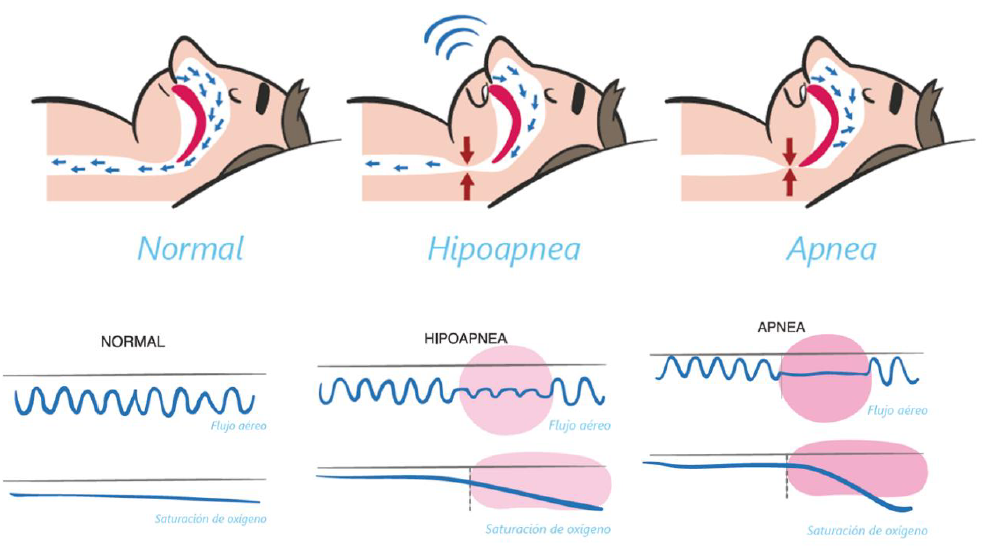
\includegraphics[width=0.75\linewidth]{img/AOS.png}
    \caption[Esquema comparativo de respiración normal, hipoapnea y apnea del sueño, junto con los respectivos patrones de flujo aéreo y saturación de oxígeno.]{Esquema comparativo de respiración normal, hipoapnea y apnea del sueño, junto con los respectivos patrones de flujo aéreo y saturación de oxígeno. Imagen adaptada de Oxigen Salud \cite{oxigensalud2025}.}
    \label{fig:AOS}
\end{figure}


\item  \textbf{Apnea Central del Sueño (ACS):} este tipo de apnea se produce por una \textbf{disfunción en el control de la respiración}, en la que el cerebro deja temporalmente de enviar señales a los músculos responsables de la respiración. A diferencia de la AOS, no existe una obstrucción física de las vías respiratorias, sino una falta de esfuerzo ventilatorio \footnote{El esfuerzo ventilatorio es la actividad muscular necesaria para permitir la entrada de aire a los pulmones.}

\item \textbf{Apnea Mixta:} combina características de la apnea central y la obstructiva. Habitualmente, un episodio comienza sin esfuerzo respiratorio (como en la apnea central) y continúa con una obstrucción de la vía aérea (como en la apnea obstructiva). Es frecuente en pacientes con formas graves de trastornos respiratorios del sueño.

\end{itemize}
El tratamiento se basa, en la mayoría de los casos, en el uso de presión positiva continua en las vías respiratorias (CPAP), que mantiene la vía aérea abierta durante el sueño y reduce los eventos de apnea. En casos leves pueden emplearse dispositivos de avance mandibular, mientras que en casos seleccionados se recurre a intervenciones quirúrgicas. Además, las modificaciones en el estilo de vida (como la pérdida de peso, evitar alcohol y sedantes y adoptar una postura adecuada al dormir) también son clave para una mejoría \cite{mayoclinic_apnea}.


\subsection{Insomnio}
El insomnio es uno de los trastornos del sueño más comunes y se manifiesta como una dificultad persistente para iniciar o mantener el sueño, o bien como un despertar temprano con incapacidad para volver a dormir. Estas alteraciones provocan un deterioro significativo en el funcionamiento diurno del individuo. La prevalencia de este trastorno oscila entre el 10\% y el 30\% de la población general, y puede llegar hasta el 50\% en grupos específicos como personas mayores o con comorbilidades psiquiátricas \cite{morin2012chronic}.

Se distinguen dos formas principales: el \textbf{insomnio agudo}, que dura días o semanas y suele estar relacionado con factores estresantes temporales; y el \textbf{insomnio crónico}, que persiste al menos tres veces por semana durante un mínimo de tres meses. 

Entre los factores de riesgo se incluyen el estrés crónico, trastornos de ansiedad y depresión, enfermedades médicas (como dolor crónico, enfermedad pulmonar obstructiva crónica o insuficiencia cardíaca), así como hábitos de sueño irregulares, uso de estimulantes y envejecimiento \cite{ninds_narcolepsy}.

Para su diagnóstico, se utilizan cuestionarios estandarizados como el \textbf{Índice de Severidad del Insomnio (ISI)}, registros de sueño y diarios del sueño. En casos concretos, pueden utilizarse técnicas adicionales como la \textbf{actigrafía} o la \textbf{polisomnografía}, especialmente si se sospecha la presencia de otros trastornos del sueño asociados, como la apnea \cite{ISI}.


\subsection{Narcolepsia}
La narcolepsia es un trastorno neurológico crónico que afecta la regulación del sueño-vigilia. Se caracteriza por una \textbf{somnolencia diurna excesiva} y episodios involuntarios de sueño. Otros síntomas clásicos incluyen cataplejía (pérdida súbita del tono muscular desencadenada por emociones), \textbf{alucinaciones hipnagógicas e hipnopómpicas} y \textbf{parálisis del sueño} \cite{ninds_narcolepsy}.

Se reconocen dos tipos principales: la \textbf{narcolepsia tipo 1}, asociada con cataplejía y niveles bajos de hipocretina-1 en el líquido cefalorraquídeo \footnote{La hipocreatina es una proteína que influye en el funcionamiento del cerebro, concretamente en el mantenimiento de los ciclos sueño-vigilia. \href{https://sebbm.es/moleculas-de-la-vida/hipocretina/}{Consultar para más información}.}, y la \textbf{tipo 2}, sin cataplejía y con niveles normales de hipocretina. Su prevalencia es baja (0.02\%–0.05\%), pero el impacto en la calidad de vida del paciente es significativo \cite{mayoclinic_apnea}.

El diagnóstico se basa en la combinación de polisomnografía nocturna y el Test de Latencia Múltiple del Sueño (MSLT), que evalúa la tendencia a quedarse dormido durante el día y la aparición temprana del sueño REM.

El tratamiento se centra en el control sintomático, combinando fármacos estimulantes para la somnolencia y antidepresivos para la cataplejía, junto con estrategias conductuales como las siestas programadas \cite{pabon2010narcolepsia}.

   


\subsection{Parasomnias}

Las \textbf{parasomnias} constituyen un grupo diverso de trastornos del sueño caracterizados por la aparición de comportamientos anormales, percepciones sensoriales inusuales o experiencias desagradables durante las transiciones entre el sueño y la vigilia, así como dentro de las distintas fases del sueño. Entre las manifestaciones más frecuentes se encuentran el \textbf{sonambulismo}, los \textbf{terrores nocturnos}, las \textbf{pesadillas recurrentes} y la \textbf{parálisis del sueño}.

Estos eventos pueden ocurrir tanto durante el sueño de ondas lentas (fase N3) como durante el sueño REM, o en los periodos de transición entre estos estados. Aunque son más comunes en la infancia y, en la mayoría de los casos, tienden a ser benignos y autolimitados, en la edad adulta pueden estar asociados a factores como \textbf{trastornos del estado de ánimo}, \textbf{uso de fármacos}, \textbf{estrés crónico} o \textbf{privación del sueño}.

El diagnóstico se basa principalmente en una \textbf{historia clínica detallada}, con especial énfasis en la descripción de los episodios por parte del propio paciente o de testigos, como familiares o convivientes. En situaciones clínicas más complejas, o cuando existe la sospecha de comportamientos potencialmente peligrosos durante el sueño, puede ser necesaria la realización de una \textbf{polisomnografía nocturna con videograbación}, que permite correlacionar eventos motores con las fases del sueño y descartar otros trastornos asociados \cite{singh2018parasomnias}.



\subsection{Síndrome de Piernas Inquietas (SPI)}
El \textbf{Síndrome de Piernas Inquietas (SPI)} es un trastorno neurológico caracterizado por una \textbf{necesidad urgente e incontrolable de mover las piernas}, generalmente debido a sensaciones incómodas o molestas. Estas sensaciones suelen aparecer durante los periodos de descanso o inactividad, especialmente en la noche, lo que interfiere con el inicio y mantenimiento del sueño. Aunque su causa exacta no se conoce, se asocia con factores genéticos, deficiencia de hierro y ciertas condiciones médicas como insuficiencia renal\footnote{La insuficiencia renal es una afección en la que los riñones pierden la capacidad de filtrar los desechos y el exceso de líquidos de la sangre de forma eficaz.} o neuropatías periféricas\footnote{Las neuropatías periféricas son trastornos que afectan a los nervios periféricos, causando síntomas como dolor, hormigueo, entumecimiento o debilidad, especialmente en manos y pies.}. El tratamiento incluye cambios en el estilo de vida, suplementación de hierro si es necesario, y en algunos casos, el uso de medicamentos específicos \cite{ninds_spi}.

\section{Variables clínicas, demográficas y del estilo de vida}
Los trastornos del sueño no solo están condicionados por factores fisiológicos o neurológicos, sino que también se ven influenciados por una amplia variedad de variables clínicas, demográficas y conductuales. Comprender el papel que desempeñan estas variables resulta esencial tanto para el diagnóstico como para el desarrollo de modelos predictivos eficaces basados en datos. En este apartado se describen las principales características recogidas en el estudio, destacando su relevancia clínica y su asociación con la calidad del sueño y los trastornos más comunes.

\subsection{Variables clínicas}
\subsubsection{Índice de Masa Corporal}
El IMC es una medida utilizada para clasificar el estado nutricional de una persona, calculada como el peso dividido entre la altura.

\begin{equation}
    \text {IMC}=\frac{\text { Peso (kg)}}{\text {Altura (m)}^2} 
\end{equation}

Según la Organización Mundial de la Salud (OMS)\footnote{Obesidad y sobrepeso según la OMS \cite{oms_obesidad_2024}.}, un IMC inferior a 18.5 se considera bajo peso, entre 18.5 y 24.9 peso normal; entre 25 y 29.9 sobrepeso; y 30 o más obesidad.
\begin{table}[H]
\centering
\begin{tabular}{|l|c|}
\hline
\textbf{Categoría} & \textbf{IMC (kg/m\textsuperscript{2})} \\
\hline
Bajo peso & < 18.5 \\
Peso normal & 18.5 – 24.9 \\
Sobrepeso & 25.0 – 29.9 \\
Obesidad & $\geq 30.0$ \\
\hline
\end{tabular}
\caption{Clasificación del IMC según la OMS.}
\label{tab:clasificacion_imc}
\end{table}


La obesidad se ha identificado como un factor de riesgo clave para la apnea obstructiva del sueño, debido al efecto del tejido adiposo en la obstrucción de las vías respiratorias superiores.

 \subsubsection{Presión Arterial}
 La presión arterial es la fuerza que ejerce la sangre contra las paredes de las arterias y se expresa en milímetros de mercurio (mmHg) mediante dos valores: sistólica (máxima) y diastólica (mínima).

 Los valores normales en adultos son aproximadamente 120/80 mmHg. Valores superiores a 140/90 mmHg indican hipertensión\footnote{\href{https://enfermeriaencardiologia.com/salud-cardiovascular/prevencion/factores-de-riesgo/presion-arterial}{Valores de referencia de presión arterial.}}, un trastorno que se ha relacionado con una menor calidad del sueño y mayor prevalencia de apnea obstructiva.

 El control de la presión arterial es crucial en personas con trastornos del sueño, ya que se ha evidenciado una asociación entre apnea no tratada y daño cardiovascular a largo plazo.

 \subsubsection{Frecuencia cardíaca}
 La frecuencia cardíaca (FC) representa el \textbf{número de latidos del corazón por minuto} y es un indicador clave del estado de salud cardiovascular. En adultos sanos en reposo, la FC suele situarse entre 60 y 100 latidos por minuto. Valores persistentemente por encima de este rango (taquicardia) pueden estar relacionados con estrés, ansiedad, enfermedades cardiovasculares o mala calidad del sueño, mientras que valores bajos (bradicardia) pueden observarse en personas entrenadas o con trastornos del ritmo cardíaco \cite{heartRate}.

Durante el sueño, la FC tiende a disminuir debido al predominio del tono parasimpático, especialmente en las fases profundas del sueño NREM. Sin embargo, durante la fase REM puede observarse una mayor variabilidad. Las alteraciones del patrón nocturno de frecuencia cardíaca han sido estudiadas como posibles marcadores de trastornos del sueño como la apnea o el insomnio.

\subsubsection{Saturación de Oxígeno (SpO$_2$)}

La saturación de oxígeno en sangre (SpO\textsubscript{2}) representa el porcentaje de hemoglobina arterial que se encuentra unida al oxígeno. Es un indicador clave del estado respiratorio y se mide comúnmente mediante pulsioximetría, una técnica no invasiva basada en fotopletismografía (PPG).

Los valores normales de SpO$_2$ en adultos sanos oscilan entre el 95\% y el 100\% en reposo. Valores por debajo del 90\% indican hipoxemia y pueden estar relacionados con patologías como la apnea del sueño, enfermedades pulmonares o insuficiencia cardíaca.

Aunque esta variable no está incluida en el conjunto de datos utilizado para entrenar el modelo predictivo, en el presente trabajo se ha registrado de forma externa mediante el dispositivo O2Ring, lo que ha permitido validar empíricamente los resultados del modelo sobre casos reales.

\begin{table}[H]
\centering
\label{tab:variables_clinicas}
\begin{tabular}{|l|c|}
\hline
\textbf{Variable} & \textbf{Valores normales} \\
\hline
Presión arterial & 120/80 mmHg \\
Índice de Masa Corporal (IMC) & 18.5–24.9 kg/m\textsuperscript{2} \\
Saturación de oxígeno (SpO\textsubscript{2}) & 95\%–100\% \\
Frecuencia cardíaca (FC) & 60-100 ppm \\
\hline
\end{tabular}
\caption{Valores de referencia para variables clínicas.}
\end{table}



\subsection{Variables demográficas}
\subsubsection{Edad}
La edad es uno de los principales factores que afectan a la calidad del sueño. Con el envejecimiento, se observa una disminución progresiva del sueño profundo (fase N3), una mayor fragmentación del descanso y un incremento en la latencia para conciliar el sueño. Además, la edad avanzada se ha asociado con una mayor prevalencia de trastornos como el insomnio crónico y la apnea obstructiva del sueño \cite{MADRID-VALERO2017}. 



\subsubsection{Género}
El género también influye en la prevalencia y manifestación de los trastornos del sueño. En general, las mujeres reportan con mayor frecuencia dificultades para iniciar o mantener el sueño, mientras que los hombres presentan una mayor incidencia de apnea obstructiva del sueño. Estas diferencias pueden explicarse por factores hormonales, anatómicos y conductuales \cite{krishnan2006gender}.

\subsubsection{Ocupación}
La ocupación laboral tiene un impacto directo en los ritmos circadianos y la calidad del descanso. Profesiones que implican turnos nocturnos, rotaciones frecuentes o niveles elevados de estrés se han asociado con insomnio, fatiga crónica y somnolencia diurna excesiva. La alteración del ritmo sueño-vigilia en trabajadores por turnos representa un factor de riesgo reconocido para múltiples alteraciones del sueño \cite{varma2025understanding}.


\subsection{Variables del estilo de vida}
\subsubsection{Duración del sueño}
Corresponde al número de horas que una persona duerme por noche. La National Sleep Foundation recomienda entre 7 y 9 horas para adultos\footnote{\href{https://www.sleepfoundation.org/how-sleep-works/how-much-sleep-do-we-really-need}{National Sleep Foundation – How Much Sleep Do We Really Need? (2024)}.}. Dormir menos de 6 horas o más de 9 de forma persistente se ha asociado con un mayor riesgo de alteraciones metabólicas, deterioro cognitivo y trastornos del estado de ánimo\footnote{\href{https://doi.org/10.1016/j.smrv.2017.11.001}{Kredlow et al., 2018. Sleep medicine reviews}.}.


\subsubsection{Calidad del sueño}
La calidad del sueño es una medida subjetiva que recoge la percepción general de la persona sobre su descanso. Incluye factores como facilidad para conciliar el sueño, número de despertares, sensación de descanso al despertar o presencia de sueños vividos.

Una baja calidad del sueño se asocia con insomnio, apnea del sueño o estrés crónico.


\subsubsection{Nivel de estrés}
El estrés activa el eje hipotálamo–hipófisis–adrenal, lo que incrementa la secreción de cortisol\footnote{El cortisol es una hormona producida por las glándulas suprarrenales en respuesta al estrés.}. Esta respuesta fisiológica puede dificultar la conciliación del sueño y disminuir su profundidad. Cuando el estrés se prolonga en el tiempo, puede desencadenar insomnio crónico \cite{nivel_estres}.


\subsubsection{Actividad física y pasos diarios}
El ejercicio regular, especialmente el aeróbico, se ha relacionado con mejoras en la eficiencia del sueño y una reducción de los síntomas de insomnio. El conteo de pasos diarios actúa como un indicador objetivo del nivel de actividad física y se ha propuesto como un parámetro útil en estudios de estilo de vida saludable \cite{efectoActividad}.


\noindent
Todas las variables clínicas, demográficas y de estilo de vida descritas en este apartado han sido consideradas como posibles predictores en el desarrollo del modelo multiclase. Su elección se ha basado tanto en evidencia clínica como en su disponibilidad accesible, permitiendo construir un sistema interpretable y aplicable en contextos no hospitalarios. 



\section{Técnicas de Evaluación del Sueño}
El estudio de la calidad del sueño requiere herramientas y metodologías que permitan evaluar sus características fisiológicas y subjetivas de manera fiable. Tradicionalmente, el diagnóstico de los trastornos del sueño ha dependido de técnicas de monitorización en entornos clínicos, como la \textbf{polisomnografía (PSG)}, considerada el estándar de referencia. Sin embargo, en los últimos años han surgido \textbf{métodos alternativos} que permiten evaluar la calidad del sueño en entornos domiciliarios, como la \textbf{poligrafía respiratoria}, la \textbf{actigrafía}, la \textbf{pulsioximetría nocturna} y diversos cuestionarios de autoinforme.

Este apartado revisa los principales técnicas utilizadas para la evaluación del sueño, agrupándolas en técnicas clínicas, dispositivos portátiles y herramientas subjetivas de autoinforme.

\subsection{Métodos Clínicos}
\subsubsection{Polisomnografía (PSG)}
La \textbf{polisomnografía (PSG)} es la técnica más completa para el estudio del sueño y se considera el método de referencia en el diagnóstico de trastornos como la apnea del sueño, la narcolepsia o el insomnio de origen neurológico. Consiste en el registro simultáneo de múltiples variables fisiológicas durante una noche completa de sueño en un laboratorio especializado.

Los parámetros evaluados incluyen:

\begin{itemize}
    \item \textbf{Electroencefalograma (EEG):} mide la actividad eléctrica cerebral y permite la identificación de las fases del sueño.
    \item \textbf{Electrooculograma (EOG):} registra los movimientos oculares, esenciales para identificar la fase REM.
    \item \textbf{Electromiografía (EMG):} analiza la actividad muscular en el mentón y extremidades, útil para detectar trastornos motores asociados al sueño.
    \item \textbf{Monitorización cardiorrespiratoria:} sensores de flujo aéreo, bandas torácicas y pulsioxímetros permiten detectar apneas e hipoapneas.
    \item \textbf{Registro de la posición corporal y movimientos:} proporciona información sobre eventos respiratorios relacionados con la postura.
\end{itemize}
Pese a su precisión, la PSG presenta limitaciones importantes: su elevado coste, la necesidad de realizarla en un entorno clínico y la posible alteración del sueño del paciente debido al monitoreo en laboratorio (\textbf{efecto de primera noche}) \cite{polisomnografia}\cite{martin2025practicas}.

Por ello, su uso como prueba de cribado poblacional es inviable, lo que motiva la búsqueda de alternativas más accesibles.

\subsubsection{Poligrafía Respiratoria (PR)}
La \textbf{poligrafía respiratoria} es una alternativa simplificada a la PSG, utilizada principalmente en la detección de apnea obstructiva del sueño. A diferencia de la PSG, no evalúa la actividad cerebral ni las fases del sueño, sino que se centra en variables cardiorrespiratorias como el flujo de aire, la saturación de oxígeno y el esfuerzo respiratorio.

La principal ventaja de la poligrafía es su \textbf{accesibilidad} y la posibilidad de su realización en el domicilio del paciente, evitando los costos y las molestias de la hospitalización. Sin embargo, su menor capacidad para diferenciar los distintos tipos de apnea y la ausencia de datos neurológicos limitan su uso en la evaluación de otros trastornos del sueño \cite{collop2007clinical}.

\subsection{Tecnologías Portátiles}

\subsubsection{Actigrafía}
La \textbf{actigrafía} es un método no invasivo basado en un acelerómetro de muñeca que mide los movimientos del paciente a lo largo de varios días o semanas para estimar los patrones de sueño-vigilia. Este dispositivo registra la actividad motora y la exposición a la luz, permitiendo inferir los periodos de sueño y vigilia con una precisión aceptable en individuos sin trastornos graves del sueño \cite{actigrafia}.

Es una herramienta útil en la evaluación de insomnio y ritmos circadianos, ya que permite comparar la percepción subjetiva del paciente con los datos objetivos del dispositivo. No obstante, presenta limitaciones en la detección de despertares nocturnos y en la diferenciación entre sueño ligero y vigilia en pacientes con baja movilidad \cite{actigrafia2013}.

Su carácter no invasivo y de uso domiciliario la convierten en una herramienta complementaria útil en la práctica clínica y en entornos de investigación longitudinal.

\subsubsection{Dispositivos portátiles y Pulsioximetría Nocturna}

La \textbf{pulsioximetría} es una técnica no invasiva basada en el uso de sensores ópticos que emplean luz roja e infrarroja para estimar la saturación de oxígeno en sangre (SpO$_2$) y la frecuencia cardíaca. Esta tecnología se basa en el principio de la fotopletismografía (PPG), que permite detectar cambios en el volumen sanguíneo mediante la absorción diferencial de luz por la hemoglobina oxigenada y desoxigenada.

\begin{figure}[H]
    \centering
    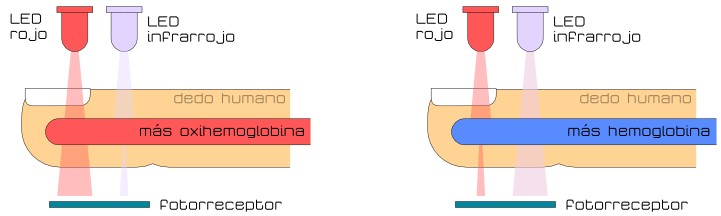
\includegraphics[width=0.9\linewidth]{img/funcionamiento-oxímetro-pulsómetro.png}
    \caption[Esquema de funcionamiento de un pulsioxímetro.]{Esquema de funcionamiento de un pulsioxímetro.\\ 
    Fuente: \cite{ventura2024monitorizacion}.}
    \label{fig:pulsioximetro}
\end{figure}

Los dispositivos portátiles o \textit{wearables} que incorporan esta tecnología se han popularizado como herramientas de cribado y autoseguimiento del sueño. Entre ellos se incluyen relojes inteligentes, anillos biométricos, bandas de muñeca y sensores integrados en colchones. Su funcionamiento se basa en la recolección de parámetros como el movimiento, la frecuencia cardíaca, la variabilidad del ritmo cardíaco, la temperatura corporal o la saturación de oxígeno. Entre los principales tipos de dispositivos destacan:

\begin{itemize}
    \item \textbf{Relojes inteligentes y pulseras de actividad:} como Fitbit, Garmin o Apple Watch, permiten registrar fases del sueño, ritmo cardíaco y actividad diaria. Su precisión es moderada y varía según el fabricante.
    \item \textbf{Anillos inteligentes:} como el \textit{Oura Ring}, combinan sensores de temperatura, frecuencia cardíaca y movimiento para analizar el sueño y la recuperación física.
    \item \textbf{Sensores bajo el colchón:} como el \textit{Withings Sleep Analyzer}, detectan ronquidos, movimientos y eventos respiratorios.
    \item \textbf{Pulsioxímetros nocturnos:} como el O2Ring, monitorizan continuamente la saturación de oxígeno y la frecuencia cardíaca durante el sueño mediante fotopletismografía.
\end{itemize} 
Aunque presentan limitaciones en la estimación de las fases del sueño o en la precisión de ciertos parámetros, su facilidad de uso y bajo coste los convierte en herramientas útiles para la detección preliminar de trastornos como el insomnio o la apnea del sueño.

\newpage
\textbf{O2Ring}

El \textbf{O2Ring} es un anillo inteligente desarrollado por la empresa \textit{\href{https://www.viatomtech.com/po2?lang=es}{Viatom}} que permite monitorizar de forma continua durante el sueño dos variables clave: la saturación de oxígeno en sangre (SpO\textsubscript{2}) y la frecuencia cardíaca. Su diseño compacto y cómodo lo convierte en una herramienta accesible para la detección domiciliaria de alteraciones respiratorias nocturnas, como apneas o desaturaciones.

Utiliza tecnología de \textbf{fotopletismografía (PPG)}, basada en la emisión de luz infrarroja y roja, que es absorbida de forma diferente por la hemoglobina oxigenada y desoxigenada. Esta propiedad permite estimar de manera precisa el porcentaje de oxígeno en sangre y la frecuencia cardíaca del usuario mientras duerme.

\begin{figure} [H]
    \centering
    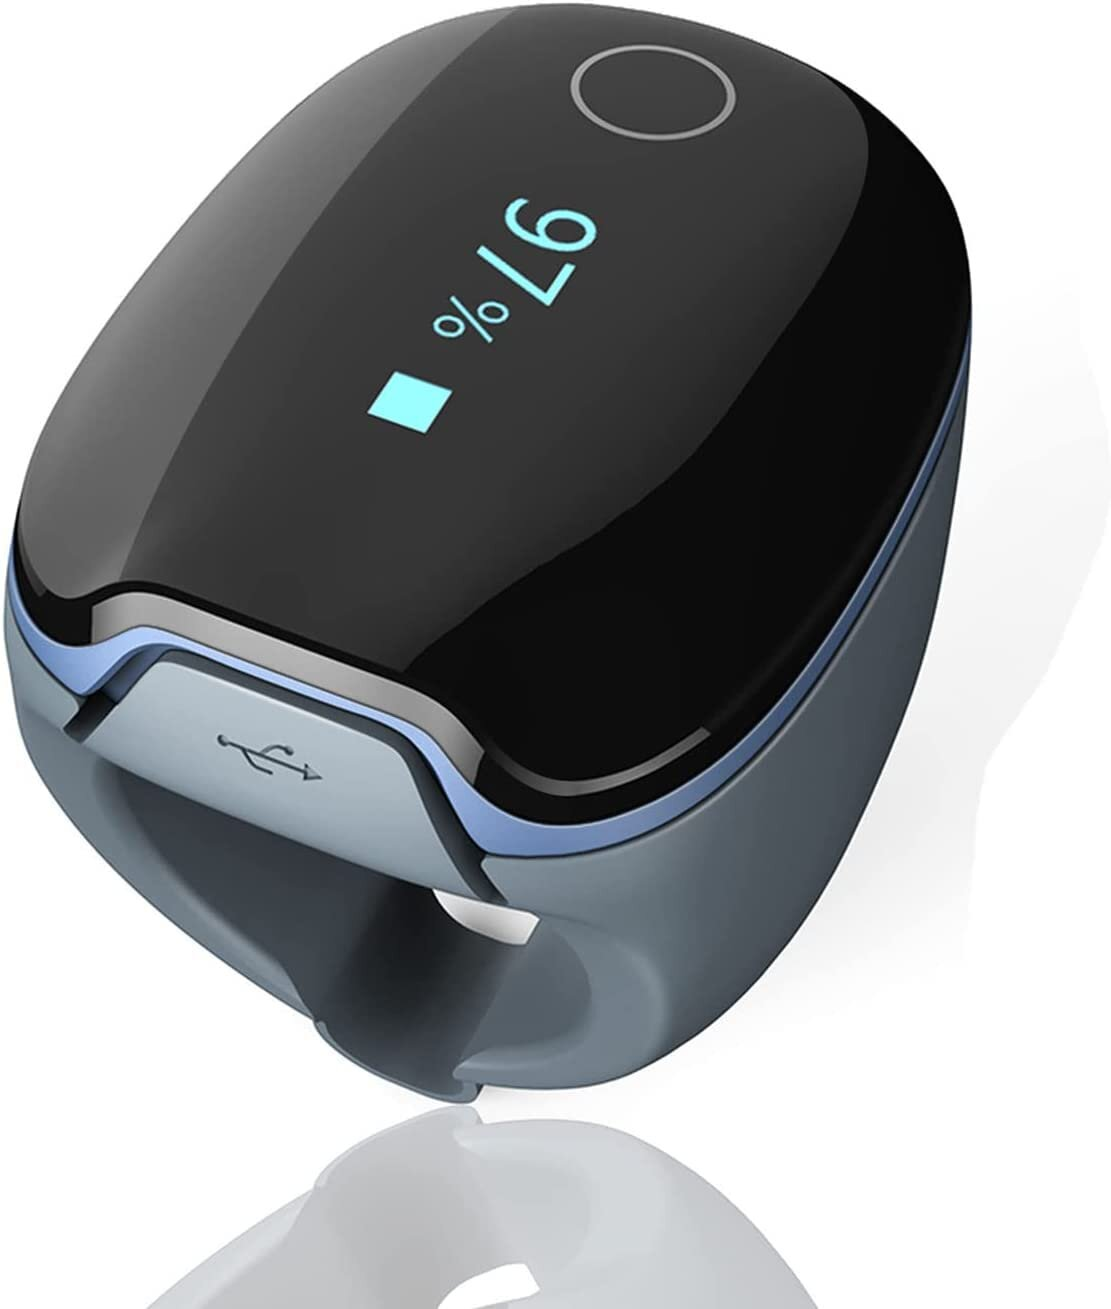
\includegraphics[width=0.25\linewidth]{img/o2ring.jpg}
    \caption[Dispositivo O2Ring de Viatom.]{Dispositivo O2Ring de Viatom. Fuente: \cite{o2ring_ifdesign}.}
    \label{fig:o2ring}
\end{figure}

Entre sus características principales destacan:
\begin{itemize}
    \item Registro continuo y no invasivo de SpO\textsubscript{2} y frecuencia cardíaca.
    \item Alertas por vibración ante desaturaciones significativas.
    \item Sincronización con apps móviles y exportación de informes en PDF o CSV.
    \item Generación de métricas como el índice de desaturación de oxígeno (ODI) o el tiempo con SpO\textsubscript{2} por debajo del 90\%.
\end{itemize}

A nivel clínico, el O2Ring se ha validado como herramienta útil en el \textit{screening}\footnote{El término \textit{screening} hace referencia a un proceso de cribado o detección precoz, que permite identificar posibles enfermedades en personas aparentemente sanas mediante pruebas rápidas, accesibles y no invasivas.} de apnea del sueño leve o moderada, especialmente en casos donde no se dispone de una polisomnografía completa. También permite un seguimiento longitudinal de pacientes y una evaluación complementaria a métodos tradicionales.

No obstante, presenta limitaciones: no ofrece información sobre las fases del sueño, ni detecta apneas centrales ni distingue entre tipos de eventos respiratorios. Por tanto, debe utilizarse como complemento y no como sustituto de un diagnóstico clínico completo.

En este trabajo, el O2Ring se ha utilizado como herramienta auxiliar para validar perfiles clínicos. Las métricas extraídas de sus informes (como caídas sostenidas de SpO$_2$, frecuencia cardíaca elevada y valores anómalos de ODI) permitieron reforzar la evaluación del modelo predictivo frente a situaciones clínicas reales.


\subsection{Cuestionarios Subjetivos}

\subsubsection{Índice de Calidad del Sueño de Pittsburgh (PSQI)}

El \textbf{Pittsburgh Sleep Quality Index (PSQI)} es un cuestionario ampliamente utilizado para evaluar la calidad subjetiva del sueño en el último mes. Consiste en 19 ítems agrupados en siete componentes: calidad subjetiva, latencia del sueño, duración, eficiencia, despertares nocturnos, uso de medicación y somnolencia diurna \cite{buysse1989pittsburgh}.

Su facilidad de aplicación y su validez en la detección de trastornos del sueño lo convierten en una herramienta útil tanto en investigación como en práctica clínica \cite{mollayeva2016pittsburgh}. Sin embargo, al basarse en autoinforme, puede estar sujeto a \textbf{sesgos de percepción} y variabilidad interindividual.

\subsubsection{Índice de Gravedad del Insomnio (ISI)}
El \textbf{Índice de Gravedad del Insomnio (ISI)} es un cuestionario diseñado específicamente para evaluar la severidad del insomnio. Se compone de siete ítems que valoran la dificultad para iniciar y mantener el sueño, la interferencia con la vida diaria y la preocupación del paciente por sus problemas de sueño \cite{ISI}.

El ISI es una herramienta eficaz para el diagnóstico y seguimiento del insomnio, aunque su uso es complementario a otros métodos, ya que no permite identificar causas orgánicas subyacentes.

\subsubsection{Escala de Somnolencia de Epworth (ESS)}
La \textbf{Escala de Somnolencia de Epworth (ESS)} mide la propensión del individuo a quedarse dormido en diversas situaciones diurnas, como leer, ver televisión o viajar como pasajero. Su puntuación permite detectar somnolencia excesiva, siendo útil en la evaluación de apnea del sueño y narcolepsia \cite{epworth}.

Si bien es una herramienta sencilla y fiable, la ESS es una medida subjetiva y no sustituye a pruebas objetivas como la PSG o el Test de Latencia Múltiple del Sueño (MSLT) \cite{pedrozo2020estructura}.

\subsubsection{Escala de Somnolencia de Stanford (SSS)}
La \textbf{Escala de Somnolencia de Stanford (SSS)} permite medir el nivel de alerta en distintos momentos del día mediante una escala de 1 a 7. Se utiliza en estudios sobre privación de sueño y trastornos de vigilia \cite{stanford}. Aunque es útil para evaluar la somnolencia en tiempo real, su aplicación es más limitada en comparación con otras herramientas subjetivas de evaluación del sueño.

\noindent
En conjunto, las herramientas descritas conforman un ecosistema amplio para la evaluación del sueño, que va desde técnicas clínicas de alta precisión hasta métodos accesibles y subjetivos. En este trabajo, se ha optado por un enfoque centrado en datos autodeclarados y medidas clínicas básicas, complementado con la validación externa mediante pulsioximetría. Esta combinación busca maximizar la accesibilidad del sistema predictivo sin comprometer su rigor diagnóstico.


\section{Aprendizaje automático (Machine Learning) en medicina}

El aprendizaje automático (Machine Learning, ML) es una rama de la inteligencia artificial que desarrolla algoritmos capaces de aprender patrones a partir de datos y realizar predicciones o decisiones sin estar explícitamente programados para cada tarea. En el contexto médico, su uso ha crecido de forma exponencial debido al aumento del volumen de datos clínicos disponibles y a la necesidad de herramientas que faciliten su análisis e interpretación.

Entre sus principales aplicaciones en el ámbito de la salud destacan:

\begin{itemize}
    \item \textbf{Diagnóstico asistido}: identificación de enfermedades a partir de imágenes médicas, señales fisiológicas o datos clínicos estructurados\footnote{\href{https://doi.org/10.1038/s41591-018-0337-2}{Guía para el aprendizaje profundo en el ámbito sanitario.}}.
    \item \textbf{Pronóstico de enfermedades}: predicción de la evolución clínica de un paciente, el riesgo de complicaciones o la respuesta esperada a un tratamiento.
    \item \textbf{Medicina personalizada}: adaptación de estrategias terapéuticas en función de las características genéticas, clínicas o conductuales del paciente.
    \item \textbf{Gestión hospitalaria}: optimización de flujos de trabajo, recursos sanitarios y toma de decisiones administrativas.
\end{itemize}

El uso de modelos de ML en medicina plantea, no obstante, desafíos importantes. Entre ellos destacan la necesidad de trabajar con datos clínicos de calidad, garantizar la equidad en las predicciones para evitar sesgos, y asegurar que los modelos sean interpretables, especialmente en entornos clínicos donde las decisiones deben ser justificadas de forma transparente.


\subsection{Modelos predictivos}
Los modelos predictivos son herramientas estadísticas y computacionales que permiten anticipar eventos futuros o clasificar instancias a partir de patrones aprendidos de datos. En el ámbito de la salud, estos modelos se emplean para prever la aparición de enfermedades, evaluar riesgos clínicos y apoyar la toma de decisiones médicas, especialmente en contextos como la predicción de trastornos del sueño.

A continuación, se describen algunos de los modelos más empleados en aprendizaje automático supervisado, todos ellos utilizados en este trabajo para predecir la presencia de trastornos del sueño a partir de variables clínicas y de estilo de vida.


\subsubsection{Regresión Logística}
La \textbf{regresión logística} es un modelo de clasificación (binaria o multiclase) que estima la probabilidad de pertenencia a una clase utilizando la función sigmoide. Se basa en la regresión lineal, pero transforma su salida en valores entre 0 y 1 mediante la función logística, que son interpretables como probabilidades:


\begin{equation}
    P(Y=1 \mid X)=\frac{1}{1+e^{-\left(\beta_{0}+\beta_{1} X_{1}+\ldots+\beta_{n} X_{n}\right)}}
\end{equation}
Donde $\beta$ representa los coeficientes del modelo, estimados mediante máxima verosimilitud. La regresión logística se utiliza ampliamente en medicina por su bajo coste computacional, facilidad de implementación e interpretabilidad de los resultados \cite{datatab_logistic_regression}.

\begin{figure}[H]
    \centering
    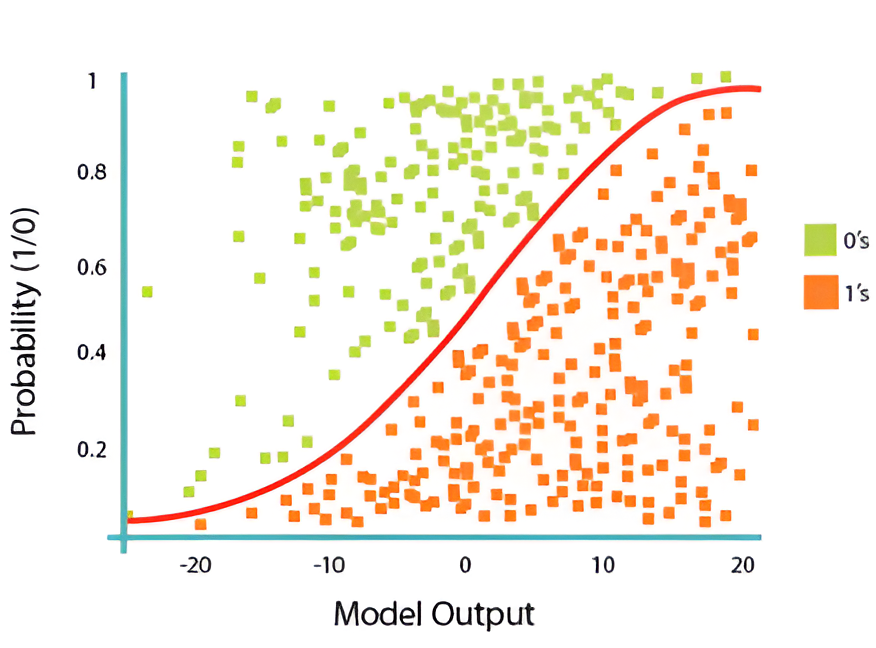
\includegraphics[width=0.5\linewidth]{img/regresionLogistica.png}
    \caption[Representación de la curva sigmoide en un modelo de regresión logística binaria.]{Representación de la curva sigmoide en un modelo de regresión logística binaria. Fuente: \cite{rafael2024ml}.}
    \label{fig:regresion_logistica}
\end{figure}

Su transparencia y la interpretación directa de los coeficientes hacen que la regresión logística sea especialmente adecuada en entornos clínicos donde se requiere justificar cada decisión de forma comprensible para el personal médico.

\subsubsection{Árboles de Decisión}

Los árboles de decisión dividen el espacio de características en regiones homogéneas mediante divisiones sucesivas. Cada nodo representa una condición sobre una variable, y las ramas conducen a clases específicas. El criterio de impureza más utilizado es el índice de Gini:


\begin{equation}
    Gini=1-\sum_{i=1}^{C} p_{i}^{2}
\end{equation}
 
donde $p_i$ es la proporción de observaciones de la clase $i$ en el nodo. Este modelo es especialmente útil en medicina por su capacidad explicativa y visual. Sin embargo, sufre de sobreajuste, por lo que suele combinarse con técnicas de ensamblado como Random Forest \cite{datacamp_decision_tree}.

\begin{figure}[H]
    \centering
    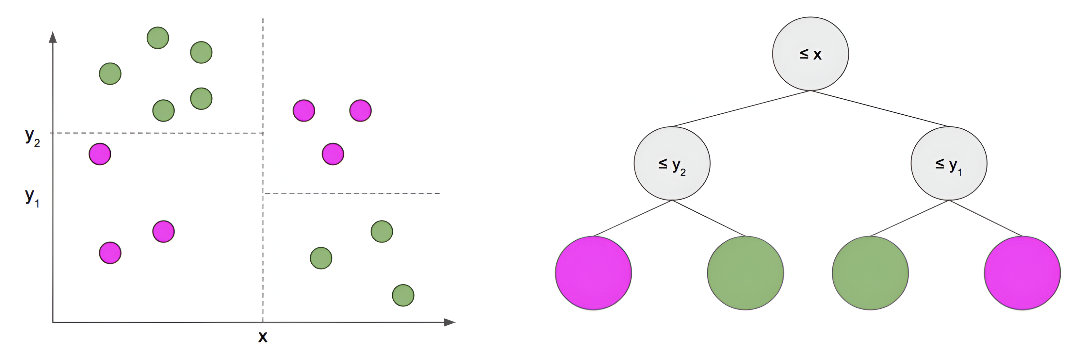
\includegraphics[width=0.7\linewidth]{img/decision_tree.png}
    \caption[Ejemplo ilustrativo del funcionamiento de un árbol de decisión.]{Ejemplo ilustrativo del funcionamiento de un árbol de decisión. Fuente: \cite{orellana2018arboles}.}
    \label{fig:decision-tree}
\end{figure}

Pese a su sencillez, los árboles de decisión ofrecen una visualización directa del proceso de toma de decisiones, siendo útiles tanto en fase exploratoria como en modelos base para técnicas más robustas como Random Forest.

\subsubsection{Máquinas de Vectores de Soporte}

Las \textbf{SVM} son modelos supervisados que buscan un hiperplano óptimo que separe las clases maximizando el margen entre ellas. Su formulación para el caso lineal es:


\begin{equation}
    \max _{\mathbf{w}, b} \frac{1}{\|\mathbf{w}\|} \quad \text { sujeto a } \quad y_{i}\left(\mathbf{w} \cdot \mathbf{x}_{i}+b\right) \geq 1, \forall i
\end{equation}
Donde w es el vector normal al hiperplano y b es el sesgo. 

En casos no lineales, se emplean funciones kernel (como RBF) para proyectar los datos a un espacio de mayor dimensión. Las SVM son ampliamente utilizadas en biomedicina para tareas de clasificación sobre señales fisiológicas \cite{ibm_svm}. 

\begin{figure}[H]
    \centering
    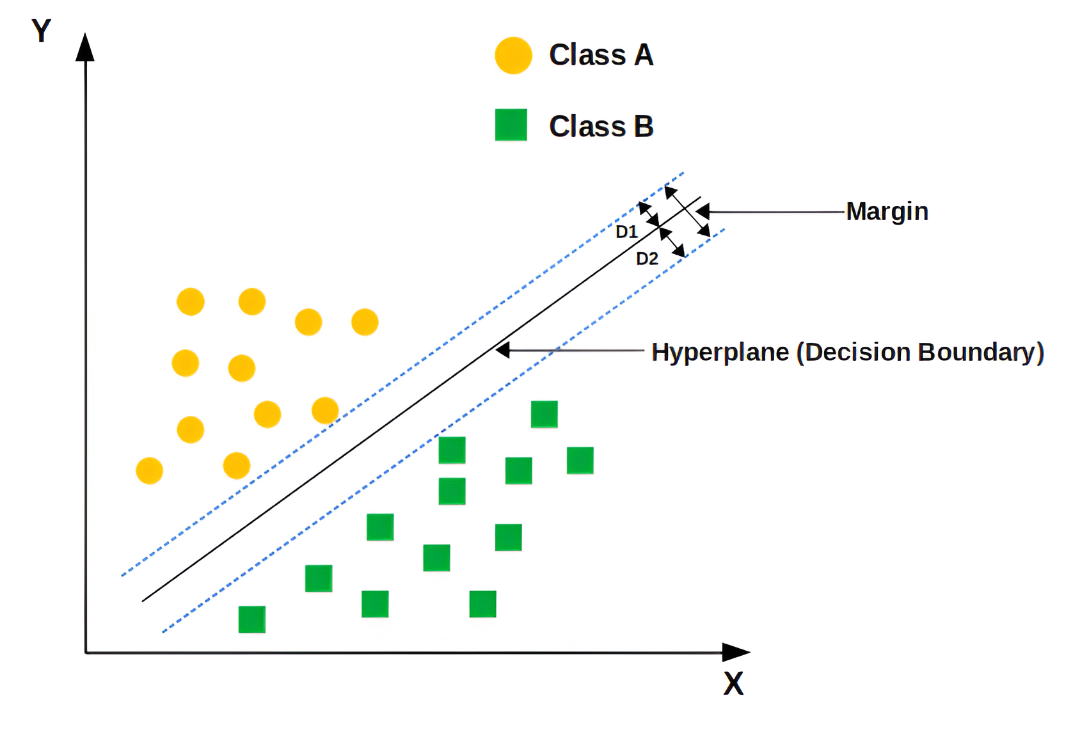
\includegraphics[width=0.8\linewidth]{img/svm.png}
    \caption[Imagen representativa del funcionamiento de SVM.]{Imagen representativa del funcionamiento de SVM.\\ Fuente: \cite{mehta2021svm}.}
    \label{fig:svm}
\end{figure}

Sin embargo, su coste computacional aumenta significativamente con el tamaño del conjunto de entrenamiento y la necesidad de ajustar adecuadamente el kernel y sus parámetros puede limitar su aplicabilidad práctica en tiempo real.

\subsubsection{Perceptrón Multicapa (MLP)}
El\textbf{ MLP} es un tipo de red neuronal que consta de una capa de entrada, una o más ocultas y una de salida. Cada neurona aplica una función de activación a una combinación ponderada de las entradas:

\begin{equation}
    h_{j}=f\left(\sum_{i=1}^{n} w_{j i} x_{i}+b_{j}\right)
\end{equation}
Donde w\textsubscript{ji }son los pesos sinápticos y b\textsubscript{j} es el sesgo. 

Este modelo se entrena por retropropagación del error, utilizando algoritmos de descenso de gradiente. En medicina, se emplea para la clasificación de EEG, oximetría y otros biomarcadores \cite{ibm_mlp}.

\begin{figure}[H]
    \centering
    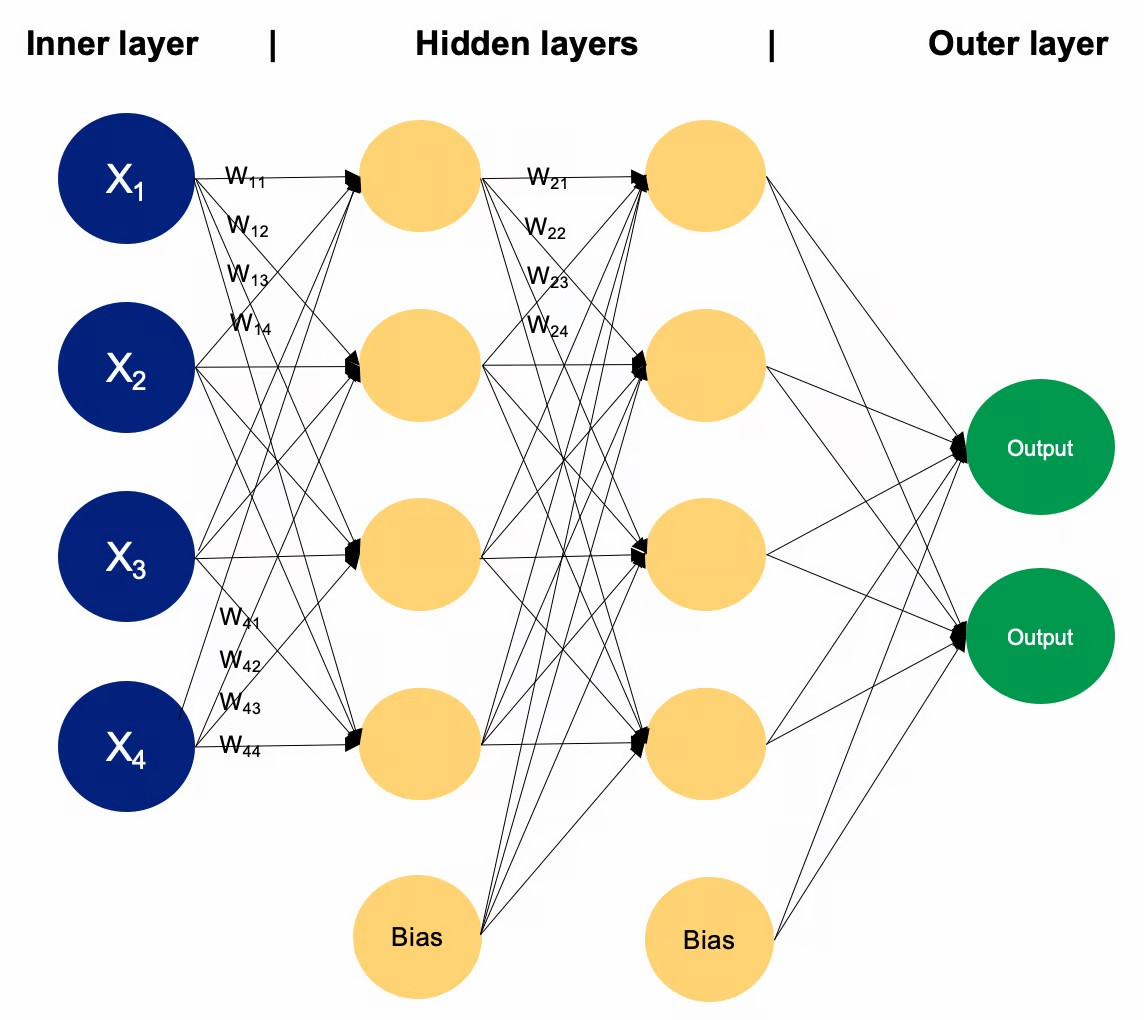
\includegraphics[width=0.8\linewidth]{img/mlp.jpg}
    \caption[Imagen representativa del funcionamiento de MLP.]{Imagen representativa del funcionamiento de MLP.\\ Fuente: \cite{mlp}.}
    \label{fig:mlp}
\end{figure}

\subsubsection{Random Forest}
\textbf{Random Forest} es un algoritmo de ensamblado que combina múltiples árboles de decisión entrenados con subconjuntos aleatorios del conjunto de datos y características (bagging). La predicción final se obtiene por votación mayoritaria:

\begin{equation}
    \hat{y}=\operatorname{modo}\left(T_{1}(x), T_{2}(x), \ldots, T_{n}(x)\right)
\end{equation}
Donde T\textsubscript{i}(x) es la predicción del i-ésimo árbol. Este enfoque mejora la generalización y reduce el sobreajuste. En medicina, ha demostrado buen rendimiento en la detección de apnea del sueño y otras condiciones clínicas complejas \cite{ibm_random_forest}.

\begin{figure}[H]
    \centering
    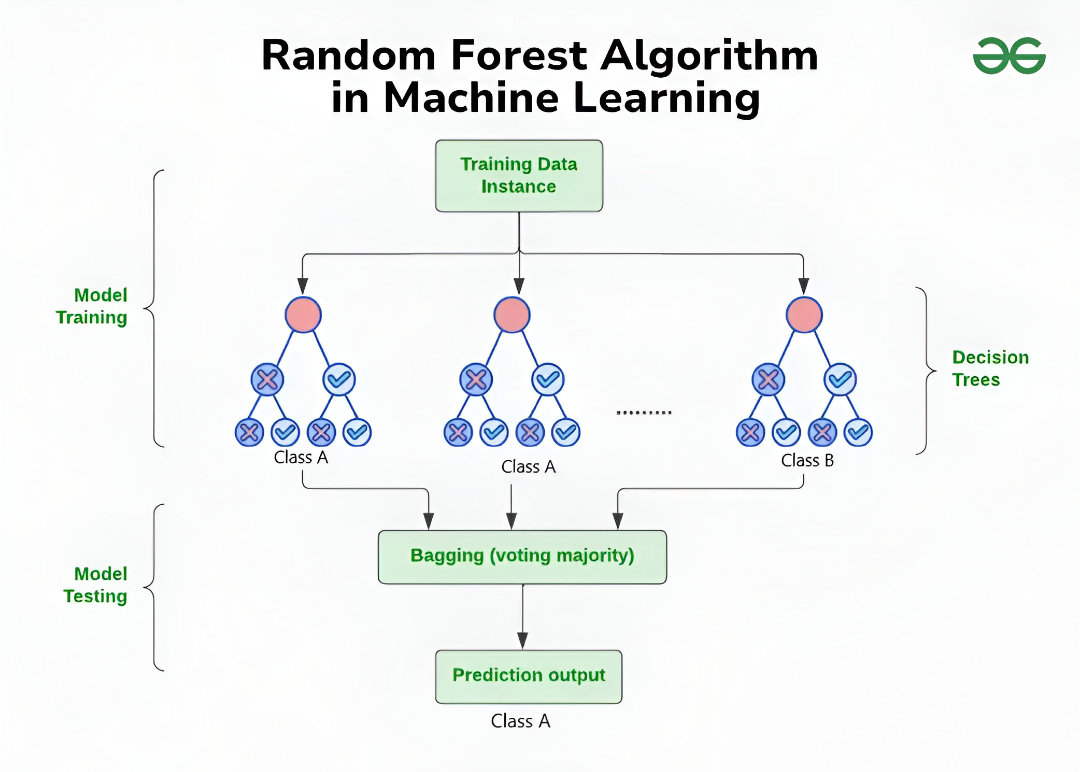
\includegraphics[width=0.8\linewidth]{img/randomForest.jpg}
    \caption[Imagen representativa del funcionamiento de Random Forest.]{Imagen representativa del funcionamiento de Random Forest. Fuente: \cite{random_forest}.}
    \label{fig:rf}
\end{figure}
Su robustez frente al sobreajuste y su capacidad para manejar datos heterogéneos lo convierten en un candidato idóneo para modelos clínicos en los que se combinan variables fisiológicas, demográficas y del estilo de vida, como en el presente trabajo.

\section{Desbalanceo de clases y técnica SMOTE}

En problemas de clasificación médica, especialmente en contextos de cribado o detección precoz, es habitual que algunas clases, como la presencia de una patología, estén infrarrepresentadas respecto a la clase mayoritaria. En el caso de los trastornos del sueño, por ejemplo, suele haber más registros de personas sin patología que de pacientes con insomnio o apnea, lo que dificulta que los modelos aprendan patrones representativos de las clases minoritarias.

Este desequilibrio puede inducir una falsa sensación de buen rendimiento basada únicamente en la exactitud global, mientras que el modelo falla sistemáticamente en identificar los casos clínicamente relevantes (baja sensibilidad).

Para mitigar este problema, una de las técnicas más utilizadas es el \textit{Synthetic Minority Over-sampling Technique} (SMOTE), propuesta por \cite{chawla2002smote}. SMOTE genera nuevas instancias sintéticas de la clase minoritaria mediante interpolación entre ejemplos reales, evitando el sobreajuste que provoca el simple duplicado de muestras. De este modo, se logra una representación más equilibrada del espacio de características.

Su aplicación ha demostrado mejorar métricas clave como la sensibilidad y el F1-score en tareas de clasificación médica sobre conjuntos de datos desbalanceados \cite{fernandez2018smote}. No obstante, en problemas multiclase puede introducir ruido si las fronteras entre clases están poco definidas, por lo que su uso debe ser evaluado cuidadosamente.

En este trabajo, se ha evaluado el impacto de aplicar SMOTE en combinación con distintos algoritmos, comparando su rendimiento frente a versiones no balanceadas del modelo. Se ha observado una mejora significativa en la sensibilidad de las clases minoritarias (insomnio y apnea), lo que justifica su uso controlado en la fase de entrenamiento.

Una vez mitigado el desbalance entre clases, resulta fundamental garantizar que las decisiones del modelo sean comprensibles y justificables desde un punto de vista clínico. Por este motivo, se han aplicado técnicas de interpretabilidad como SHAP.

\section{Interpretabilidad del modelo: SHAP}

En el desarrollo de modelos predictivos aplicados a la medicina, la interpretabilidad es una condición indispensable para garantizar transparencia diagnóstica y confianza por parte de los profesionales. A diferencia de los modelos lineales, muchas técnicas avanzadas de aprendizaje automático —como los ensamblados o las redes neuronales— actúan como cajas negras, dificultando la explicación de las decisiones individuales del sistema.

Entre las técnicas más consolidadas para interpretar este tipo de modelos destaca SHAP (\textit{SHapley Additive exPlanations}), una metodología basada en los valores de Shapley de la teoría de juegos cooperativos \cite{shap}. SHAP permite descomponer cada predicción en contribuciones atribuibles a cada variable de entrada, cuantificando la influencia de cada una sobre el resultado final.

Las principales ventajas de SHAP en contextos clínicos incluyen:

\begin{itemize}
  \item \textbf{Validación del modelo:} permite verificar que las decisiones se basan en relaciones clínicas coherentes y no en correlaciones espurias.
  \item \textbf{Generación de confianza:} facilita la aceptación del sistema por parte de los profesionales, al ofrecer una explicación intuitiva y detallada de cada recomendación.
  \item \textbf{Detección de sesgos:} ayuda a identificar variables con un impacto indebido sobre la salida del modelo, revelando posibles fuentes de discriminación o error.
  \item \textbf{Medicina personalizada:} permite adaptar la interpretación del modelo al perfil específico de cada paciente, favoreciendo decisiones individualizadas.
\end{itemize}

En el presente trabajo, SHAP se ha utilizado para analizar tanto la importancia media de cada predictor como su contribución específica a cada observación. Por ejemplo, en ciertos perfiles clínicos simulados, SHAP mostró que variables como la ocupación laboral, el nivel de estrés y la duración del sueño tenían más peso que el IMC en la predicción de insomnio. Esta capacidad de explicación local y global convierte a SHAP en una herramienta clave para garantizar la trazabilidad y justificación de las decisiones clínicas basadas en el modelo.


\section{Aplicaciones web interactivas en Ciencia de Datos}
En el contexto del aprendizaje automático y la ingeniería biomédica, las aplicaciones web interactivas permiten acercar los modelos predictivos al usuario final de manera accesible, visual y funcional. Estas herramientas actúan como una capa de interfaz entre los algoritmos complejos desarrollados durante la fase de entrenamiento y el profesional sanitario o paciente que desea obtener información personalizada a partir de ellos.

\subsection{Interfaz como puente entre el modelo y el usuario}
Una aplicación interactiva permite al usuario introducir variables relevantes (como edad, presión arterial, nivel de estrés, calidad del sueño, etc.) y recibir una predicción automática y explicable generada por el modelo, sin necesidad de conocimientos técnicos. Esta predicción puede estar acompañada de explicaciones visuales, indicadores de riesgo o recomendaciones, lo que mejora la interpretabilidad de los resultados y su utilidad clínica.

En ingeniería de la salud, estas herramientas tienen un alto potencial: pueden contribuir al cribado poblacional, al apoyo en la toma de decisiones clínicas o al autocuidado en poblaciones con riesgo de enfermedades crónicas. La posibilidad de utilizar estas aplicaciones desde cualquier dispositivo con conexión a internet facilita, además, la democratización del acceso a tecnologías basadas en inteligencia artificial.

\subsection{Streamlit como herramienta de desarrollo}
Streamlit es un framework de código abierto en Python diseñado específicamente para crear aplicaciones web interactivas orientadas a la ciencia de datos y el aprendizaje automático \cite{streamlit}. Su sintaxis sencilla permite transformar scripts de análisis en interfaces web funcionales sin necesidad de conocimientos avanzados de desarrollo frontend.

Entre sus características principales destacan:
\begin{itemize}
    \item \textbf{Facilidad de uso}: permite crear interfaces web con pocas líneas de código.
    \item \textbf{Compatibilidad}: se integra de forma nativa con bibliotecas populares como \textit{Pandas}, \textit{scikit-learn}, \textit{Matplotlib} o \textit{SHAP}.
    \item \textbf{Interactividad}: permite actualizar los resultados en tiempo real conforme el usuario introduce nuevos datos.
\end{itemize}

Gracias a estas ventajas, Streamlit se presenta como una solución ideal para prototipado rápido, aplicaciones ligeras o proyectos académicos. En el presente trabajo, se ha utilizado para desarrollar una aplicación interactiva que permite introducir datos personales, realizar una predicción automática del tipo de trastorno del sueño (si lo hubiera) y visualizar las variables que han contribuido a dicha decisión. Esta estrategia refuerza la transparencia y confiabilidad del sistema, facilitando su adopción tanto por profesionales clínicos como por usuarios finales sin conocimientos de programación.

El desarrollo de esta interfaz mediante Streamlit ha sido clave para trasladar el modelo predictivo desde un entorno experimental hacia una herramienta funcional, explicable y accesible, en línea con las necesidades de los sistemas de salud actuales.


\section{Estado del arte y trabajos relacionados}

\subsection{Aplicación del aprendizaje automático al estudio del sueño}

En los últimos años, el uso de modelos de aprendizaje automático (ML) para el estudio del sueño ha cobrado gran relevancia, tanto en el ámbito clínico como en el desarrollo de soluciones portables y accesibles. Estas técnicas permiten desarrollar sistemas predictivos no invasivos, capaces de analizar grandes volúmenes de datos clínicos y autodeclarados con fines de cribado o apoyo diagnóstico.

Ha et al. (2023) desarrollaron un modelo basado en \textit{XGBoost} para predecir la presencia de apnea del sueño (OSA), insomnio o COMISA, utilizando variables clínicas y autodeclaradas. La herramienta, denominada \textit{SLEEPS}, alcanzó un AUC superior a 0.89 en todos los modelos, y fue desplegada como una aplicación web accesible, integrando explicaciones mediante \textit{SHAP} \cite{ha2023sleeps}. Este enfoque es conceptualmente similar al adoptado en el presente trabajo, aunque aquí se ha optado por un modelo Random Forest con calibración, interpretabilidad visual y exportación de informes.

Otro estudio relevante es el de Alazaidah et al. (2023), que realizaron una comparación exhaustiva entre modelos de regresión y clasificación aplicados a la predicción de trastornos del sueño. Su análisis evidencia el potencial del aprendizaje automático para detectar condiciones como insomnio o apnea mediante variables clínicas, sociodemográficas y de estilo de vida \cite{alazaidah2023potential}.


\subsection{Modelos centrados en la predicción de calidad del sueño}

Además de los enfoques clínicos tradicionales, diversos estudios han explorado la predicción de la calidad del sueño desde una perspectiva continua, empleando dispositivos portátiles y variables fisiológicas.

Sathyanarayana et al. (2016) desarrollaron modelos de redes neuronales para predecir la calidad del sueño (medida en términos de eficiencia) utilizando únicamente los datos recogidos durante el día por dispositivos portátiles. Este enfoque destaca por evitar la necesidad de medir parámetros nocturnos, y por lograr resultados robustos en tareas de clasificación binaria entre “sueño bueno” y “sueño pobre” \cite{sathyanarayana2016sleep}.

De forma similar, Kilic et al. (2023) entrenaron modelos de \textit{convolutional neural networks} y \textit{ensemble learning} utilizando el conjunto de datos NetHealth, que incluye registros de 698 estudiantes universitarios. Obtuvieron resultados prometedores en la clasificación binaria de calidad del sueño, utilizando variables como la actividad física, el nivel de estrés y datos recogidos por sensores portátiles. Estos hallazgos destacan el potencial de los enfoques basados en dispositivos cotidianos para aplicaciones de salud digital \cite{wearablesCNN}.

En un contexto más fisiológico, Di Credico et al. (2024) utilizaron biofeedback (variabilidad de la frecuencia cardíaca, temperatura cutánea) para estimar la calidad del sueño, validándolo contra el índice de Pittsburgh (PSQI). Sus resultados confirmaron que es posible aproximar la calidad subjetiva del sueño mediante parámetros fácilmente medibles, lo cual apoya la base del presente trabajo, basado también en datos autodeclarados y clínicos \cite{di2024predicting}.

\subsection{Interpretabilidad y herramientas explicables}

Uno de los retos más relevantes en el uso de modelos de ML en medicina es la necesidad de interpretabilidad. Ahadian et al. (2024) propusieron un modelo híbrido (LSTM + TCN + Transformer) para predecir trastornos del sueño, complementado con explicaciones SHAP y contrafactuales. Su trabajo demuestra que es posible combinar precisión técnica con trazabilidad clínica \cite{ahadian2024explainable}.

En este trabajo, se ha seguido una filosofía similar al incorporar SHAP tanto en la interpretación global como individual del modelo. Esta integración permite justificar cada predicción y y presentarla de forma comprensible y justificable ante profesionales clínicos o incluso pacientes.

\subsection{Aplicaciones interactivas y despliegue accesible}

El uso de interfaces interactivas para la predicción personalizada ha sido ya validado en estudios como el de Ha et al. (2023), que despliega su modelo mediante una herramienta web que incluye visualizaciones y explicaciones automáticas. De forma complementaria, Espie et al. (2012) demostraron que una aplicación basada en terapia cognitivo-conductual (\textit{Sleepio}) era capaz de mejorar significativamente los síntomas de insomnio en ensayos clínicos aleatorizados \cite{espie2012sleepio}.

Este tipo de plataformas no solo permiten hacer llegar la predicción a la población general, sino que también facilitan el seguimiento clínico o el autodiagnóstico responsable.

El presente trabajo se sitúa en esta línea, pero con un enfoque distinto: se ha desarrollado una aplicación ligera y accesible mediante \textit{Streamlit}, que combina predicción multiclase personalizada, visualización explicativa mediante \textit{SHAP} y generación automática de informes PDF con orientación clínica. A diferencia de otras plataformas centradas en intervención terapéutica, esta herramienta busca facilitar el cribado inicial y la comunicación clara de los resultados, sin requerir conocimientos técnicos por parte del usuario final.


\subsection{Modelos basados en señales fisiológicas y pulsioximetría}

Varios trabajos recientes han explorado la posibilidad de detectar trastornos del sueño, especialmente apnea obstructiva, a partir de señales fisiológicas obtenidas mediante pulsioximetría o sensores biométricos portátiles. Estos enfoques buscan alternativas menos invasivas que la polisomnografía, apoyándose en señales como la saturación de oxígeno (SpO$_2$) y la frecuencia cardíaca (FC) registradas durante el sueño.

Gutiérrez-Tobal et al. (2020) desarrollaron un sistema basado en aprendizaje automático para la detección de apnea del sueño exclusivamente a partir de la señal de SpO$_2$. Empleando un conjunto amplio de características estadísticas y morfológicas extraídas de la pulsioximetría nocturna, validadas frente a polisomnografía, logrando una alta precisión y sensibilidad \cite{gutierrez2020apnea}.


Por otro lado, Casal et al. (2024) plantearon un enfoque aún más avanzado, integrando redes neuronales de tipo TCN (Temporal Convolutional Networks) y capas Transformer. Utilizaron como entrada señales longitudinales de pulsioximetría y aplicaron técnicas de atención para destacar los intervalos temporales más relevantes. Su modelo logró una discriminación efectiva entre sujetos control y pacientes con apnea, proponiendo además un marco explicable mediante visualización de pesos de atención \cite{casal2021tcn}.

Estos estudios refuerzan el valor de incluir variables fisiológicas reales en el desarrollo de modelos explicables. Aunque el presente trabajo no integra todavía señales en tiempo real, se ha realizado una validación preliminar con el O2Ring, sentando las bases para una futura evolución del sistema hacia una monitorización continua y más precisa de la salud del sueño.

\noindent
Los conceptos revisados en este capítulo proporcionan el marco teórico necesario para comprender los fundamentos clínicos, técnicos y computacionales del sistema desarrollado. Desde los trastornos del sueño y sus variables asociadas hasta las técnicas de aprendizaje automático, interpretabilidad y despliegue interactivo, todos los elementos descritos se integran en el diseño de un modelo predictivo explicable y accesible. En el siguiente capítulo se detallan las fases metodológicas llevadas a cabo para su implementación, evaluación y validación práctica.
